\chapter{Arquitetura de Software}
\label{cap:arquitetura-software}

A arquitetura de software corresponde ao conjunto de estruturas necessárias para raciocinar sobre um sistema, compreendendo seus elementos, as relações entre eles e as propriedades que ambos apresentam \parencite{Bass2021SAP}. Essa definição desloca a atenção da tecnologia isolada para as decisões que condicionam a evolução do produto: quais partes existem, o que cada uma pode conhecer das demais e por quais meios se comunicam. Segundo \textcite{Sommerville2018ES10}, o projeto de arquitetura estabelece a ligação entre os requisitos e a organização do sistema, razão pela qual o tema se relaciona diretamente aos requisitos do Quadro~\ref{quad:requisitos_funcionais} e do Quadro~\ref{quad:requisitos_nao_funcionais}.

Este capítulo descreve a arquitetura efetivamente identificada no \textit{Civitas}. A descrição técnica tem como base o código da \textit{branch} \texttt{main} dos repositórios \textit{civitas-backend} (\textit{commit} \texttt{e7c3f30}, de 3 de abril de 2026) e \textit{civitas-frontend} (\textit{commit} \texttt{ed79c34}, de 11 de junho de 2026) \parencite{CivitasBackend2026,CivitasFrontend2026}. Recursos presentes apenas em outras \textit{branches} são mencionados somente quando necessários para explicar uma divergência e não são apresentados como implementados. Trata-se de uma análise do código e da configuração versionados: não houve medição de desempenho, teste de intrusão nem avaliação do sistema em ambiente de produção.

\section{Arquitetura de Desenvolvimento}
\label{sec:cap6-arquitetura-desenvolvimento}

A organização estrutural de um software define como suas responsabilidades são distribuídas. \textcite{Parnas1972} demonstrou que a decomposição em módulos não deve seguir apenas a sequência de execução, mas ocultar as decisões com maior probabilidade de mudança, de modo que uma alteração permaneça contida em uma parte reduzida do sistema. Esse raciocínio fundamenta a separação de responsabilidades e a modularidade: cada componente assume um objetivo delimitado e expõe uma interface pela qual os demais o utilizam, sem depender de seus detalhes internos. Um componente, nessa perspectiva, é uma unidade substituível da solução, definida pelos serviços que oferece e pelas dependências que declara \parencite{Martin2019ArquiteturaLimpa}.

Entre os padrões recorrentes, a arquitetura em camadas agrupa funcionalidades relacionadas e faz com que cada nível utilize os serviços do nível imediatamente inferior, o que favorece a substituição localizada de partes do sistema, embora nem sempre seja simples manter uma separação rigorosa entre os níveis \parencite{Sommerville2018ES10}. Já o modelo cliente-servidor distribui a solução entre serviços e os clientes que os consomem por meio de uma rede \parencite{Sommerville2018ES10}. Quando essa comunicação ocorre pela \textit{web}, o estilo REST orienta a interação por recursos identificados, operações uniformes e requisições sem estado de sessão armazenado no servidor \parencite{Fielding2000}.

Manutenibilidade e escalabilidade são atributos de qualidade influenciados por essas decisões. A primeira diz respeito ao custo e ao risco de modificar o sistema; a segunda, à capacidade de atender a uma demanda maior mediante acréscimo de recursos \parencite{Bass2021SAP}. A adoção de um padrão não assegura esses atributos por si só, pois eles dependem da disciplina de implementação e precisam ser avaliados com medidas próprias. Por isso, as vantagens mencionadas neste capítulo são tratadas como potencial da organização adotada, e não como resultado medido.

O \textit{Civitas} adota uma arquitetura cliente-servidor composta por duas aplicações mantidas em repositórios distintos e por um banco de dados relacional. O \textit{front-end}, construído com Next.js, é responsável pela apresentação e pela interação com o usuário. O \textit{back-end}, uma API construída com ASP.NET Core, concentra as regras de negócio, a autenticação e o acesso aos dados. A persistência é realizada em PostgreSQL, sistema gerenciador de banco de dados relacional de código aberto \parencite{PostgreSQLDocs}, ao qual somente a API se conecta. A Figura~\ref{fig:cap6-arquitetura} representa essa composição.

\begin{figure}[H]
\centering
\caption{Arquitetura de desenvolvimento do Civitas}
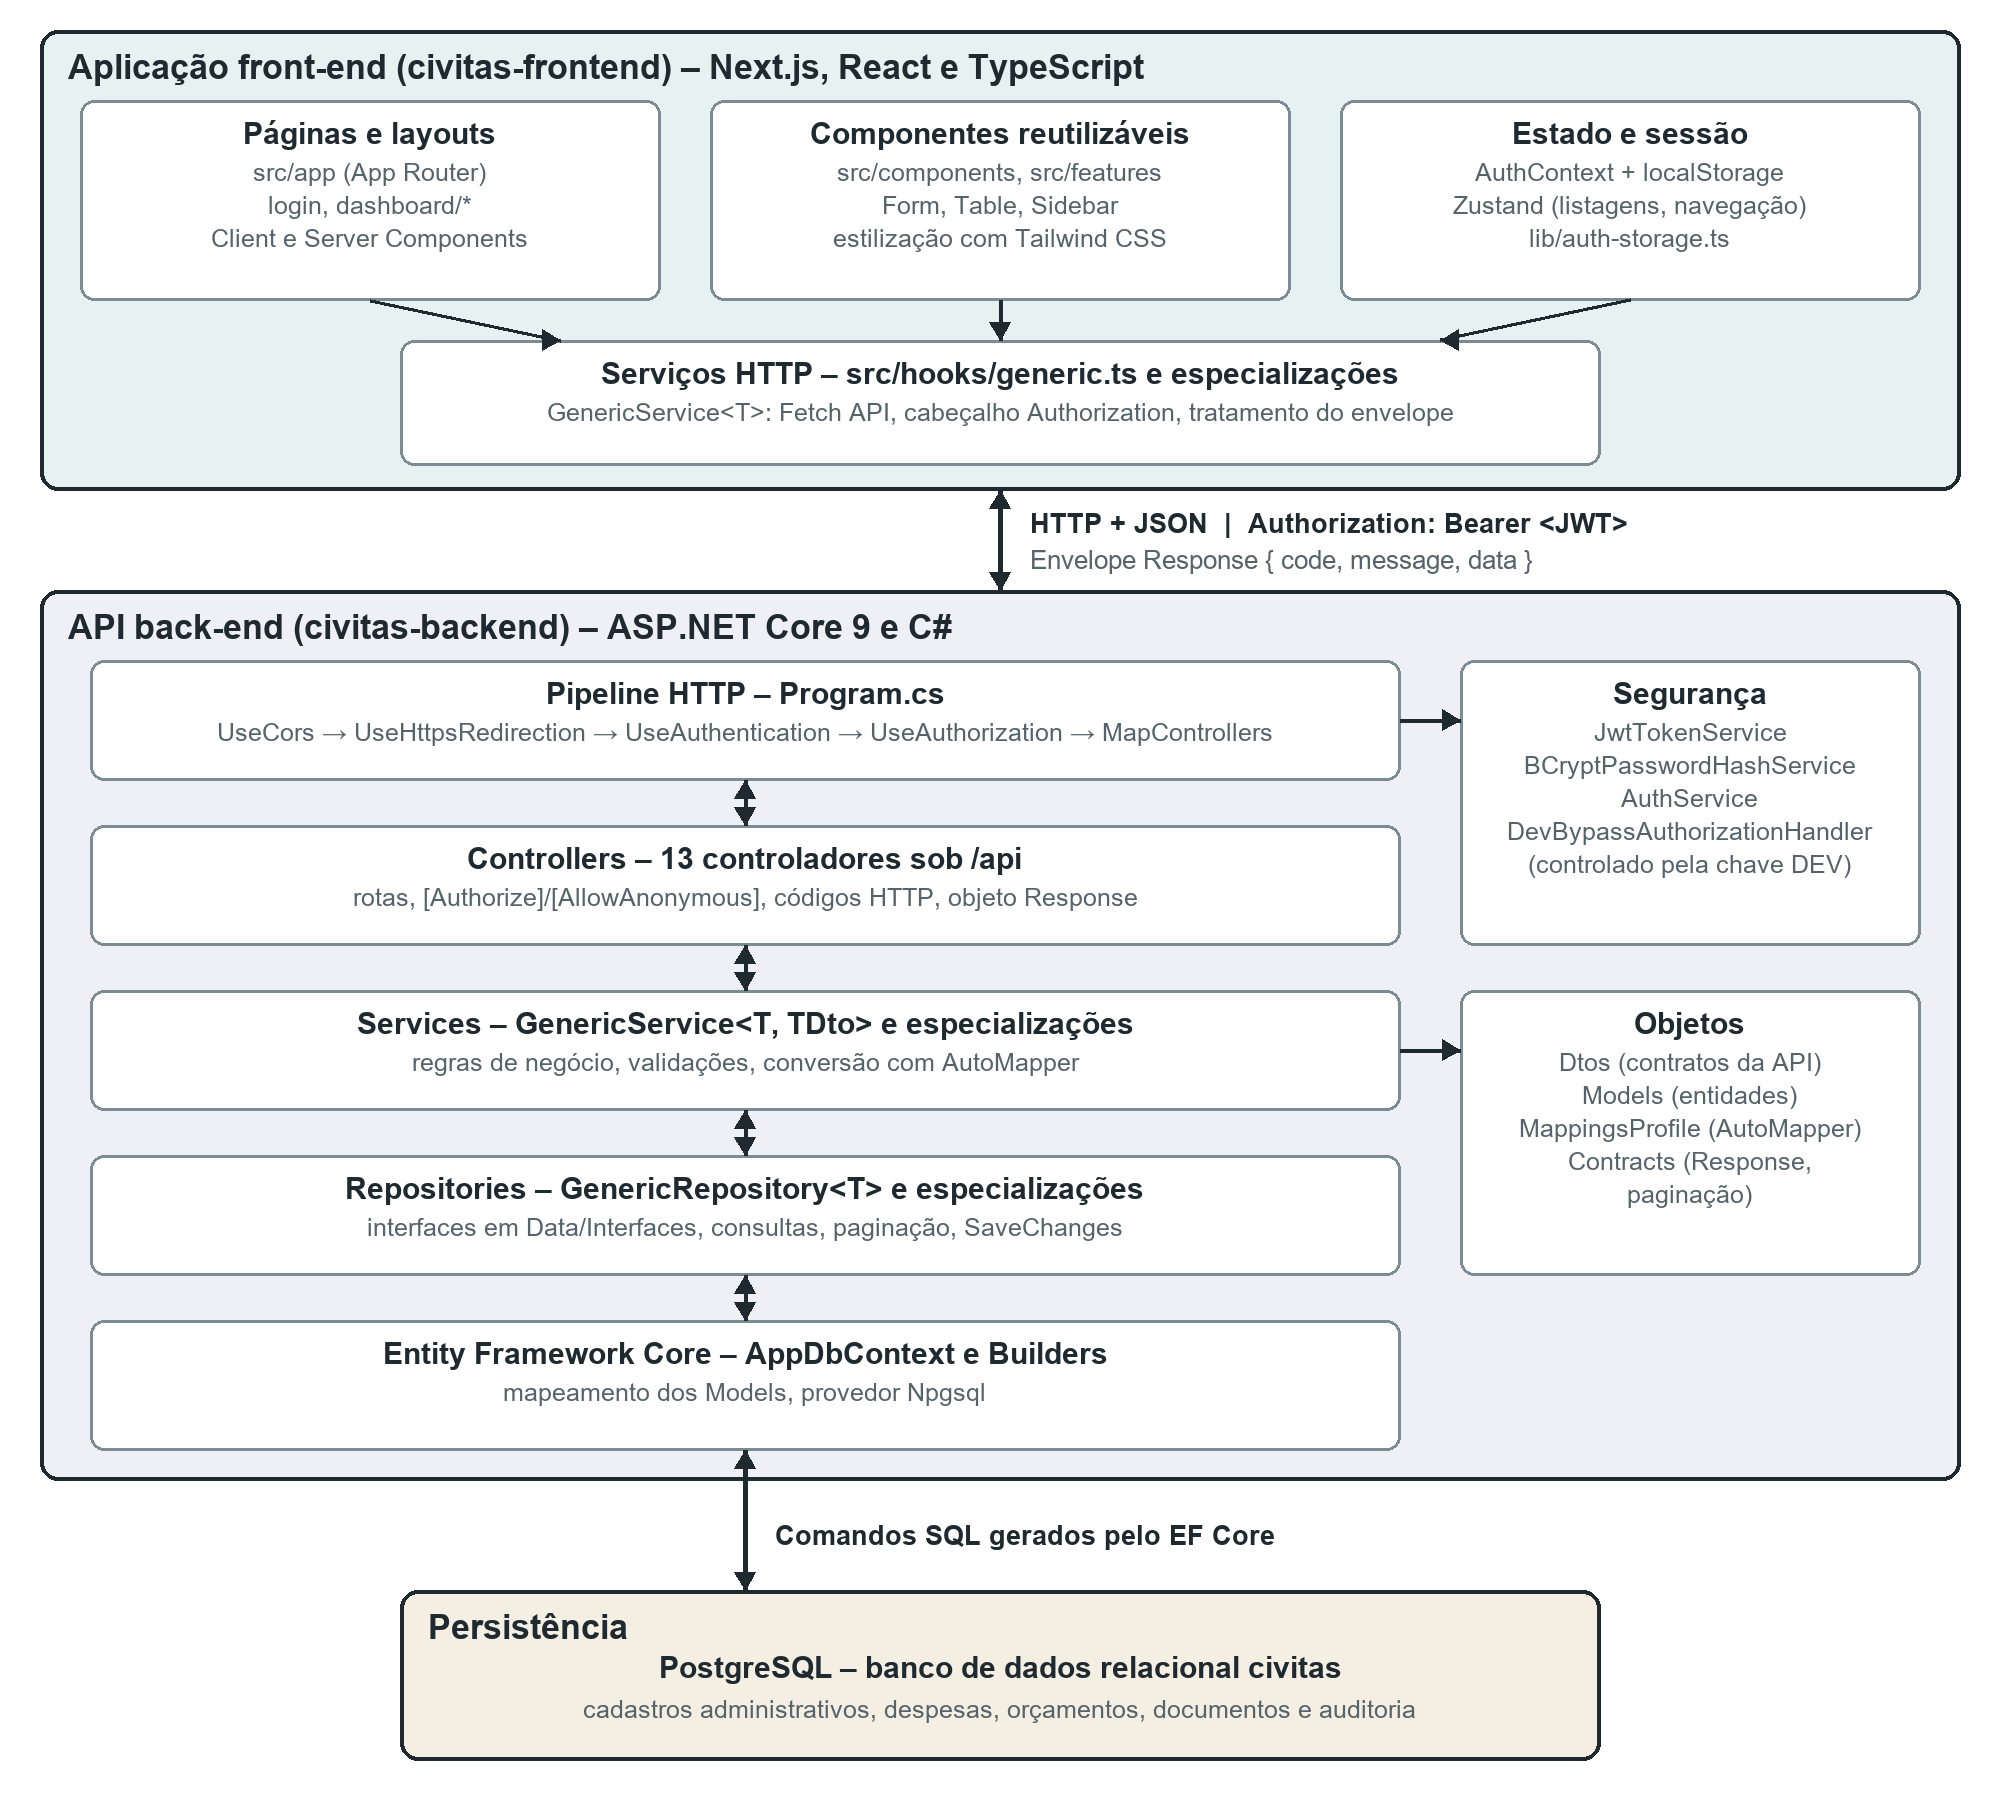
\includegraphics[width=.92\linewidth]{figs/cap6_arquitetura_civitas.png}
\label{fig:cap6-arquitetura}
\fonte{Elaborada pelos autores com base no código das \textit{branches} principais dos repositórios do Civitas.}
\end{figure}

A separação em duas aplicações atende à natureza do \textit{Civitas}, que reúne operações administrativas e financeiras sujeitas a validações e a relacionamentos entre cadastros. Com a API como único ponto de acesso aos dados, essas verificações ficam em um mesmo local, em vez de se repetirem em cada interface. A independência dos repositórios também permite que as aplicações evoluam em ritmos próprios, o que traz um custo: o contrato entre elas precisa ser mantido explicitamente, como se discute adiante nesta seção. O Quadro~\ref{qua:cap6-tecnologias} relaciona as tecnologias confirmadas nos arquivos de configuração e os respectivos pontos de uso.

\begin{quadro}[H]
\caption{Tecnologias identificadas no Civitas e sua utilização}\label{qua:cap6-tecnologias}
\small
\begin{tabularx}{\textwidth}{|P{.30\textwidth}|>{\RaggedRight\arraybackslash}X|}
\hline
\textbf{Tecnologia} & \textbf{Utilização verificada} \\ \hline
C\# e ASP.NET Core 9 & Linguagem e \textit{framework} da API (\texttt{net9.0}), com controladores e \textit{pipeline} HTTP. \\ \hline
Entity Framework Core 9 e Npgsql & Mapeamento objeto-relacional e provedor de acesso ao PostgreSQL. \\ \hline
AutoMapper & Conversão entre entidades e DTOs nas classes de serviço. \\ \hline
BCrypt.Net-Next e JWT Bearer & Geração e verificação de \textit{hash} de senhas; emissão e validação de \textit{tokens}. \\ \hline
Swashbuckle & Geração da documentação OpenAPI e da interface Swagger em ambiente de desenvolvimento. \\ \hline
xUnit e SQLite & Projeto \texttt{Civitas.WebAPI.Tests}, com testes de \textit{endpoints} sobre banco em memória. \\ \hline
Next.js 15, React 19 e TypeScript & Roteamento, renderização, componentes e tipagem do \textit{front-end}. \\ \hline
Tailwind CSS 4 & Classes utilitárias, em conjunto com variáveis definidas em \texttt{globals.css}. \\ \hline
Zustand & Estado da Central de Listagens e do indicador de progresso de navegação. \\ \hline
Fetch API & Requisições à API; a dependência Axios consta em \texttt{package.json}, mas não é importada no código. \\ \hline
ExcelJS e jsPDF & Exportação de listagens nos formatos XLSX e PDF. \\ \hline
Git, GitHub e GitHub Actions & Versionamento, \textit{pull requests} e verificação de \textit{build} do \textit{front-end}. \\ \hline
Docker & \texttt{Dockerfile} do \textit{front-end}; não há arquivo equivalente na \textit{branch} principal do \textit{back-end}. \\ \hline
\end{tabularx}
\fonte{Elaborado pelos autores com base em \texttt{Civitas.WebAPI.csproj}, \texttt{package.json} e no código-fonte.}
\end{quadro}

A integração ocorre por requisições HTTP com corpo em JSON, direcionadas às rotas sob o prefixo \texttt{/api}. O endereço base é obtido no \textit{front-end} pela variável de ambiente \texttt{NEXT\_PUBLIC\_API\_URL}, com valor padrão apontando para a porta local definida no perfil de execução da API. A autenticação ilustra o fluxo completo. A tela de \textit{login} envia e-mail e senha para \texttt{POST /api/auth/login}; a API localiza o usuário no PostgreSQL, verifica a senha e devolve um \textit{token} JWT, que o \textit{front-end} armazena no navegador. A partir daí, cada serviço HTTP inclui esse \textit{token} no cabeçalho \texttt{Authorization}, a API o valida antes de executar a ação do controlador, e a resposta retorna em um envelope padronizado, com os campos \texttt{code}, \texttt{message} e \texttt{data}, que o \textit{front-end} interpreta para apresentar dados ou mensagens.

O desenvolvimento é organizado com Git e hospedado no GitHub, na organização \textit{Fatec-ADS-AMS2025}, sendo cada aplicação um repositório próprio \parencite{ChaconStraub2014}. O histórico mostra uma \textit{branch} principal (\texttt{main}), uma \textit{branch} de integração (\texttt{dev}) e \textit{branches} de trabalho nomeadas a partir do número da tarefa e da \textit{sprint}, incorporadas por \textit{pull requests}. Os repositórios também guardam modelos de tarefa e de \textit{pull request} e documentação das entregas por \textit{sprint}, o que evidencia um trabalho organizado em ciclos sucessivos. No \textit{front-end}, um \textit{workflow} do GitHub Actions executa a instalação de dependências e o \textit{build} a cada \textit{push} ou \textit{pull request} \parencite{GitHubActionsDocs}; não foi encontrado \textit{workflow} equivalente na \textit{branch} principal do \textit{back-end}. A modelagem do domínio é mantida em arquivo da ferramenta Astah, no diretório \texttt{documentation/ClassDiagram} do repositório da API.

A análise conjunta das \textit{branches} principais revelou uma diferença de contrato que afeta a integração. O \textit{front-end}, mais recente, consome recursos que a \textit{branch} principal do \textit{back-end} não expõe, como \texttt{unidades-consumidoras} e \texttt{tipo-codigo}, além de rotas de despesas como \texttt{pagas}, \texttt{atrasadas} e \texttt{status-exclusao}, e envia despesas em \texttt{multipart/form-data}, enquanto o controlador correspondente da \texttt{main} não declara esse formato de entrada. Esses recursos existem na \textit{branch} \texttt{dev} do \textit{back-end}, que na data da análise não havia sido incorporada à \texttt{main} e também removeu os controladores de documentos e fluxos ainda presentes nesta última. Consequentemente, a arquitetura geral descrita permanece válida, mas parte das telas de despesas e de unidades consumidoras depende de uma versão da API distinta da publicada na \textit{branch} principal. A forma de operação conjunta das versões não foi verificada em execução.

\subsection{Back-End}
\label{subsec:cap6-back-end}

O \textit{back-end} é a parte do sistema executada no servidor e encarregada de receber solicitações, aplicar regras de negócio, controlar o acesso e persistir informações. Em aplicações que tratam dados administrativos e financeiros, sua importância decorre de ser um ambiente sob controle da organização: as validações executadas no navegador podem ser contornadas por um cliente modificado, de modo que as verificações determinantes precisam ocorrer no servidor \parencite{owasp2026input}. Para organizar essas responsabilidades, \textcite{Fowler2002PEAA} descreve a divisão em camadas de apresentação, domínio e fonte de dados, além de padrões como a camada de serviço e o repositório, este último também discutido por \textcite{Evans2004} como abstração que aproxima o acesso aos dados de uma coleção de objetos do domínio.

No \textit{Civitas}, o \textit{back-end} foi desenvolvido em C\#, linguagem orientada a objetos da plataforma .NET \parencite{MicrosoftCSharpTour}, com o \textit{framework} ASP.NET Core 9. A solução reúne o projeto \texttt{Civitas.WebAPI} e o projeto de testes \texttt{Civitas.WebAPI.Tests}. As camadas não são projetos compilados separadamente: são diretórios e \textit{namespaces} de uma única aplicação, separados por convenção. Os diretórios principais são \texttt{Controllers}, \texttt{Services}, \texttt{Data} e \texttt{Objects}, este último subdividido em \texttt{Models}, \texttt{Dtos}, \texttt{Enums} e \texttt{Contracts}. O arquivo \texttt{Program.cs} centraliza o registro de serviços e a composição do \textit{pipeline} de requisições, um encadeamento de componentes em que a ordem determina o tratamento aplicado \parencite{MicrosoftMiddleware}: \textit{Cross-Origin Resource Sharing} (CORS), redirecionamento para HTTPS, autenticação, autorização e, por fim, o mapeamento para os controladores.

Os controladores formam a camada de entrada. São treze classes, cada uma associada a uma rota: \texttt{api/auth}, \texttt{api/usuarios}, \texttt{api/secretarias}, \texttt{api/instituicoes}, \texttt{api/fornecedores}, \texttt{api/orcamentos}, \texttt{api/despesas}, \texttt{api/documentos}, \texttt{api/fluxos}, \texttt{api/auditorias}, \texttt{api/tipo-despesa}, \texttt{api/tipo-instituicao} e \texttt{api/unidade-medida}. O atributo \texttt{[ApiController]} ativa comportamentos próprios de APIs, como a inferência da origem dos parâmetros e a resposta automática com \textit{status} 400 quando a validação do modelo falha \parencite{MicrosoftWebApi}. Os recursos seguem um padrão semelhante: \texttt{GET} para listagem paginada e consulta por identificador, \texttt{POST} para criação, \texttt{PUT} para atualização e, na maior parte dos cadastros, \texttt{PATCH situacao/\{id\}} para alternar entre ativo e inativo, o que caracteriza exclusão lógica por meio do enumerador \texttt{Situacao}. Os controladores não acessam diretamente o banco de dados; delegam o trabalho aos serviços, recebidos por seus construtores.

A camada de serviços reúne as regras de negócio. A classe \texttt{GenericService<T, TDto>} implementa as operações comuns de consulta, paginação, criação, atualização e remoção, e as classes especializadas a estendem conforme a necessidade de cada entidade. O nível de especialização não é uniforme. \texttt{UsuarioService}, \texttt{FornecedorService}, \texttt{SecretariaService}, \texttt{DespesaService} e \texttt{AuthService} contêm validações próprias; \texttt{InstituicaoService}, \texttt{OrcamentoService}, \texttt{FluxoService}, \texttt{DocumentoService}, \texttt{TipoDespesaService}, \texttt{TipoInstituicaoService} e \texttt{UnidadeMedidaService} utilizam essencialmente o comportamento herdado, somado a consultas específicas quando existem. A camada de acesso a dados segue a mesma lógica: \texttt{GenericRepository<T>} oferece consultas sem rastreamento de alterações, filtro por enumerador, ordenação dinâmica e paginação limitada a cem registros por página, enquanto os repositórios específicos acrescentam consultas como \texttt{GetByEmailAsync} e \texttt{ExistsByNumeroDocumentoAndFornecedorAsync}. As interfaces correspondentes ficam em \texttt{Data/Interfaces} e \texttt{Services/Interfaces}.

As dependências entre as camadas são resolvidas pelo contêiner nativo de injeção de dependências do ASP.NET Core, técnica pela qual uma classe recebe seus colaboradores de um provedor externo, em vez de instanciá-los \parencite{MicrosoftDI}. Em \texttt{Program.cs}, cada interface é associada à sua implementação com tempo de vida por requisição, por meio de \texttt{AddScoped}. Assim, \texttt{DespesaService} declara a necessidade de \texttt{IDespesaRepository}, \texttt{IOrcamentoRepository} e outras abstrações sem conhecer como foram implementadas, o que também possibilita a substituição do banco de dados no projeto de testes.

Os objetos transportados pelo sistema também são separados. As classes de \texttt{Objects/Models} representam as entidades persistidas, enquanto as de \texttt{Objects/Dtos} definem os dados trocados com os clientes, seguindo o propósito do \textit{Data Transfer Object} de transportar dados entre processos \parencite{Fowler2002PEAA}. A conversão é feita pelo AutoMapper, biblioteca de mapeamento entre objetos \parencite{AutoMapperDocs}, cujas regras estão em \texttt{MappingsProfile}. Essa configuração tem efeito de segurança concreto: no mapeamento de \texttt{Usuario} para \texttt{UsuarioDTO}, o campo \texttt{Senha} é ignorado, evitando que o \textit{hash} seja devolvido nas respostas.

A persistência utiliza o Entity Framework Core, mapeador objeto-relacional da plataforma .NET \parencite{MicrosoftEFCore}, com o provedor Npgsql para PostgreSQL \parencite{NpgsqlEFCore}. A classe \texttt{AppDbContext} declara doze conjuntos de entidades (\texttt{DbSet}) e delega a configuração de cada uma às classes de \texttt{Data/Builders}, que definem chaves, tamanhos, campos obrigatórios, índices únicos e relacionamentos. Por exemplo, \texttt{UsuarioBuilder} cria índices únicos para CPF, e-mail e matrícula, e \texttt{DespesaBuilder} define chaves estrangeiras com exclusão restrita, impedindo no banco a remoção de registros referenciados. A conexão é informada na chave \texttt{DefaultConnection} da configuração da aplicação.

O recurso de \textit{migrations} permite atualizar o esquema do banco de forma incremental, mantendo-o em sincronia com o modelo \parencite{MicrosoftEFMigrations}, e está previsto no projeto pelo pacote de ferramentas e pelas instruções do \texttt{README}. Contudo, o arquivo \texttt{.gitignore} exclui o diretório \texttt{Migrations} e a \textit{branch} principal mantém nele apenas \texttt{AppDbContextModelSnapshot.cs}. Portanto, o repositório registra o estado atual do modelo, mas não o histórico de alterações necessário para que \texttt{dotnet ef database update} reconstrua o esquema a partir de um clone recente. A evolução estruturada do banco, nesse sentido, encontra-se parcialmente documentada no controle de versão.

A validação de dados combina diferentes níveis. No cadastro de usuários, \texttt{UsuarioService} normaliza os campos, valida CPF pelos dígitos verificadores, UF, CEP, formato de e-mail e composição da senha, verifica a unicidade de CPF, e-mail e matrícula e reúne os erros encontrados em uma única exceção. Atributos de validação do tipo \textit{Data Annotations} aparecem apenas em \texttt{AuditoriaDTO} e, como mencionado, parte dos serviços não possui regras próprias, ficando sujeita somente à vinculação de tipos e às restrições do banco. Portanto, a profundidade da validação varia conforme o módulo.

O cadastro de despesas exemplifica a comunicação entre as camadas. Ao receber \texttt{POST /api/despesas}, a ação \texttt{Post} de \texttt{DespesaController} chama \texttt{ValidarCadastroAsync}, de \texttt{DespesaService}. Esse método normaliza os campos; exige número de documento numérico; impede data de emissão futura e vencimento anterior à emissão; confirma a existência do tipo de despesa, do orçamento, da instituição, do fornecedor e do usuário; verifica se o orçamento pertence à instituição informada; rejeita fornecedor inativo; exige a Unidade Consumidora (UC) quando o tipo de despesa a solicita; e impede a repetição do documento para o mesmo fornecedor, consultando \texttt{DespesaRepository}. Aprovados esses critérios, o método \texttt{Create} herdado converte o DTO em entidade e \texttt{GenericRepository} a persiste por meio de \texttt{SaveChangesAsync}. Se uma regra falhar, o controlador captura \texttt{ArgumentException} e responde com \textit{status} 400.

O tratamento de respostas é feito em cada controlador, com a classe \texttt{Response}, formada por um código do enumerador \texttt{ResponseEnum}, uma mensagem e os dados, combinada aos códigos HTTP adequados, como 200, 400, 401, 404, 409 e 500. Esse formato torna previsível a interpretação pelo cliente, embora dois casos escapem ao envelope: as respostas 400 automáticas de \texttt{[ApiController]} e os erros 401 emitidos pelo próprio \textit{middleware} de autenticação. A documentação da API é gerada pelo Swashbuckle no formato OpenAPI \parencite{MicrosoftSwashbuckle}, incorporando os comentários XML do código, e a interface Swagger é habilitada apenas quando o ambiente é de desenvolvimento, com definição do esquema \textit{Bearer} para testes de rotas protegidas.

Essa organização delimita onde cada tipo de alteração deve ocorrer: uma nova rota no controlador, uma regra no serviço, uma consulta no repositório e uma restrição de esquema no \textit{builder}. As classes genéricas reduzem a repetição nos cadastros simples, o que contribui para a manutenção do \textit{Civitas}, que possui diversas entidades com operações semelhantes. Há também concessões: a repetição de blocos de tratamento de exceção nos controladores e a concentração de todas as camadas em um único projeto dependem da disciplina da equipe para preservar as fronteiras. O projeto de testes abrange autenticação, autorização, paginação e validações de usuário e fornecedor, com 26 métodos de teste declarados; como esses testes não foram executados nesta análise, sua existência não é apresentada como comprovação dos benefícios mencionados.

\subsection{Front-End}
\label{subsec:cap6-front-end}

O \textit{front-end} é a parte da aplicação com a qual o usuário interage diretamente: apresenta informações, recebe comandos e traduz as respostas do servidor em elementos compreensíveis. Em interfaces \textit{web} modernas, essa construção costuma se apoiar na componentização, que divide a tela em partes independentes e reutilizáveis, descritas como funções que combinam estrutura e comportamento \parencite{ReactComponents}. O dado que muda ao longo da interação constitui o estado, e sua organização determina a previsibilidade da interface: o estado pode pertencer a um componente, ser compartilhado por componentes próximos ou ser mantido em uma estrutura externa quando utilizado em muitas partes da aplicação \parencite{ReactManagingState}. A comunicação cliente-servidor completa esse quadro, já que o navegador obtém dados da API de forma assíncrona e atualiza apenas o necessário.

No \textit{Civitas}, a interface foi construída com Next.js 15 e React 19. O Next.js adota, no \textit{App Router}, um roteamento baseado no sistema de arquivos, em que pastas definem rotas, arquivos \texttt{page} definem páginas e arquivos \texttt{layout} definem estruturas compartilhadas \parencite{NextjsLayouts}. O código é escrito principalmente em TypeScript, verificador estático de tipos para JavaScript \parencite{TypeScriptHandbook}, com o modo estrito habilitado em \texttt{tsconfig.json}; a página \texttt{login/page.jsx} permanece em JavaScript, o que é permitido pela opção \texttt{allowJs}. A estilização combina classes utilitárias do Tailwind CSS, aplicadas diretamente na marcação \parencite{TailwindUtility}, com variáveis e classes próprias definidas em \texttt{globals.css}, nas quais se apoiam os temas e o modo de alto contraste descrito no Capítulo 4.

A organização do diretório \texttt{src} acompanha essa divisão de responsabilidades. Em \texttt{app} estão as rotas: \texttt{login}, \texttt{forgot-password} e, sob \texttt{dashboard}, as áreas de painel, Central de Listagens, configurações, despesas, fornecedores, instituições, orçamentos, perfil, secretarias, unidades consumidoras e usuários. Essas rotas correspondem às interfaces apresentadas no Capítulo 4 e aos requisitos RF14 a RF16 e RF19. Em \texttt{components} estão os elementos compartilhados, e em \texttt{hooks} estão os serviços de acesso à API e os \textit{hooks} de tela. O diretório \texttt{models} reúne os tipos das entidades, \texttt{contexts} contém o contexto de autenticação, \texttt{navigation} mantém o catálogo das áreas da aplicação utilizado na pesquisa de navegação, e \texttt{features} isola a Central de Listagens.

A componentização é visível nos módulos \texttt{Form} e \texttt{Table}. O componente de formulário recebe uma lista de campos configurados, com tipo, rótulo, máscara, obrigatoriedade, opções e seção, e assume a montagem, a validação e a normalização dos valores, o que permite reaproveitá-lo nos modos de criação, edição e visualização de vários cadastros. O módulo \texttt{Table} oferece visualizações em lista e em cartões, ordenação, ações e exportação; esta última utiliza ExcelJS e jsPDF para atender ao RF16, importados dinamicamente somente quando requisitados. Em áreas de maior complexidade, como despesas, a página delega a composição a componentes próprios, em \texttt{\_components}, e a lógica de dados a \textit{hooks} como \texttt{useDespesasDashboard}. Essa decomposição foi registrada como objetivo em documento de \textit{sprint} do repositório.

O estado é gerenciado por mecanismos diferentes, conforme o alcance. Os estados locais usam os \textit{hooks} do React, como nos campos de \texttt{login.tsx}. O estado de autenticação é compartilhado pela \textit{Context API}, em \texttt{AuthProvider}, e não pelo Zustand. Este, biblioteca de estado baseada em \textit{hooks} \parencite{ZustandDocs}, é utilizado em dois pontos: no \textit{store} da Central de Listagens, que preserva filtros, colunas e modo de visualização no \texttt{sessionStorage}, e no controle da barra de progresso de navegação, em \texttt{useNavigationProgress}. As preferências de tema e acessibilidade são mantidas em contexto e armazenamento próprios. Assim, o uso do Zustand é pontual: atende a estados compartilhados da interface, sem centralizar todo o estado da aplicação.

A comunicação HTTP é feita com a Fetch API, interface nativa para obtenção de recursos pela rede \parencite{MDNFetch}, apesar da presença do Axios entre as dependências declaradas. A classe \texttt{GenericService<T>}, em \texttt{hooks/generic.ts}, encapsula as chamadas e é especializada por classes como \texttt{DespesaService} e \texttt{FornecedorService}, cada uma associada a um recurso da API. Ela monta a URL e os parâmetros de paginação, acrescenta o cabeçalho de autorização e, em \texttt{handleResponse}, interpreta o envelope: em caso de erro, compõe uma mensagem a partir de \texttt{message} e \texttt{data}, desconsiderando chaves técnicas como \texttt{stacktrace}, e a apresenta em notificação visual; em caso de sucesso, extrai os dados ou a estrutura paginada. A exibição das respostas, portanto, é padronizada em um único ponto, o que torna coerente a forma como as telas reportam falhas. Alguns métodos auxiliares devolvem coleções vazias quando a consulta falha, o que evita a interrupção da tela, mas pode fazer com que um erro de comunicação pareça ausência de registros.

A autenticação no cliente é conduzida por \texttt{useAuth}, que envia as credenciais à API e registra os dados retornados por meio de \texttt{AuthProvider}. A sessão é persistida no \texttt{localStorage} pelo objeto \texttt{authStorage}, que descarta o registro quando o prazo informado em \texttt{expiresAtUtc} termina. A proteção das páginas é implementada em \texttt{dashboard/layout.tsx}: enquanto a sessão é restaurada, exibe-se uma mensagem de carregamento; não havendo usuário autenticado, ocorre o redirecionamento para \texttt{/login}. Trata-se de um controle executado no navegador, que orienta a navegação, mas não substitui a autorização da API. Não há arquivo de \textit{middleware} do Next.js no repositório. O encerramento da sessão remove apenas os dados locais.

Formulários e tratamento de dados envolvem etapas no cliente antes do envio. No \textit{login}, a tela verifica o preenchimento dos campos e apresenta erros junto a eles. Nos cadastros, \texttt{Input} e \texttt{lib/input-mask.ts} aplicam máscaras para dados como CPF e CNPJ, enquanto \texttt{global/formPayload.ts} converte os valores para o formato esperado. Essas verificações melhoram a resposta ao usuário, porém não dispensam as validações do servidor. A recuperação de senha merece observação: a tela existe, mas, por padrão, \texttt{useForgotPassword} simula a solicitação e somente chama a API quando uma variável de ambiente específica é habilitada, sendo que a rota correspondente não existe na \textit{branch} principal do \textit{back-end}. Da mesma forma, a tela de \textit{login} possui um atalho para \texttt{/signup}, rota sem página implementada.

A renderização também merece destaque. Por padrão, páginas e \textit{layouts} do Next.js são componentes de servidor, e APIs do navegador, como o \texttt{localStorage}, ficam disponíveis apenas em componentes de cliente \parencite{NextjsServerClient}. As páginas de usuários, fornecedores, instituições, despesas e unidades consumidoras carregam dados iniciais no servidor. Como \texttt{authStorage} retorna vazio fora do navegador, a análise estática indica que essas primeiras requisições partem sem cabeçalho de autorização e, com a proteção da API ativa, tendem a resultar em erro tratado pela própria página. Esse comportamento não foi observado em execução e deve ser examinado pela equipe.

A estrutura adotada aproxima a interface das necessidades do \textit{Civitas}: um conjunto extenso de cadastros, com padrões semelhantes de listagem e formulário, favorece componentes configuráveis e um serviço HTTP genérico. A tipagem estática explicita o formato das entidades consumidas, e o roteamento por pastas torna direta a associação entre a área funcional e seu código. Essa organização pode facilitar a manutenção à medida que novos módulos sejam incorporados, sem que isso represente, por si só, uma medida de produtividade ou qualidade.

\section{Segurança da Informação}
\label{sec:cap6-seguranca}

A segurança da informação busca preservar a confidencialidade, a integridade e a disponibilidade: respectivamente, a garantia de que a informação não seja revelada a quem não está autorizado, a manutenção de sua exatidão e completude e a possibilidade de acesso e uso sob demanda por uma entidade autorizada \parencite{ISO27000_2018}. Essas propriedades orientam a análise de riscos e dependem da combinação de medidas técnicas, processos e pessoas, não existindo mecanismo que, sozinho, as assegure \parencite{Fontes2008,Anderson2020SecEng}.

Em sistemas multiusuário, duas funções são distintas: a autenticação confirma quem está solicitando o acesso, e a autorização decide o que essa identidade pode fazer. O controle de acesso reúne as regras dessa decisão. \textcite{SaltzerSchroeder1975} formularam princípios ainda utilizados nesse campo, entre eles o menor privilégio, a verificação de cada acesso e a negação como comportamento padrão. A falha nesses controles ocupa a primeira posição na lista OWASP Top 10 de 2021 \parencite{OWASPTop10A01}, o que indica a relevância de verificar a autorização no servidor, para cada operação.

A proteção de credenciais parte de não armazenar senhas de forma recuperável. Funções de derivação como o bcrypt, proposto por \textcite{ProvosMazieres1999}, incorporam sal e custo computacional ajustável, dificultando ataques de força bruta caso a base de dados seja exposta \parencite{owasp2026password}. Na autenticação baseada em \textit{tokens}, o JSON Web Token (JWT) representa declarações em formato compacto e assinado \parencite{JonesBradleySakimura2015}, tipicamente enviadas como credencial \textit{Bearer}, de modo que quem possui o \textit{token} pode utilizá-lo; por isso, o transporte deve ser protegido e o armazenamento, cuidadoso \parencite{JonesHardt2012}. A comunicação segura costuma ser obtida com TLS, que oferece confidencialidade e integridade ao canal \parencite{RFC8446}.

Completam esse conjunto a validação das entradas, que deve ocorrer no servidor \parencite{owasp2026input}, e o registro de eventos, indispensável para auditoria e rastreabilidade: \textcite{KentSouppaya2006} destacam que os registros de segurança servem à identificação de incidentes e à investigação de atividades, desde que protegidos e geridos adequadamente. No contexto brasileiro, o tratamento de dados pessoais também está sujeito à Lei Geral de Proteção de Dados Pessoais \parencite{brasil2018lgpd}.

O \textit{Civitas} possui um mecanismo real de autenticação. O \textit{endpoint} \texttt{POST /api/auth/login}, marcado com \texttt{[AllowAnonymous]}, valida a presença de e-mail e senha; \texttt{AuthService} normaliza os valores, busca o usuário e recusa o acesso com a mesma mensagem genérica para usuário inexistente, inativo ou senha incorreta, o que evita indicar qual dessas condições ocorreu. Havendo sucesso, \texttt{JwtTokenService} gera um \textit{token} assinado com HMAC-SHA256, contendo as declarações \texttt{sub}, \texttt{name} e \texttt{tipousuario}, com validade de 60 minutos conforme a configuração. Em \texttt{Program.cs}, o \textit{middleware} JWT Bearer valida emissor, audiência, assinatura e prazo, sem tolerância adicional de relógio (\texttt{ClockSkew} igual a zero). Esses elementos estão de acordo com a parte de autenticação de RF01, RF02 e RNF-02. Não foram encontrados, contudo, \textit{refresh token}, revogação no servidor ou limitação de tentativas de \textit{login}: um \textit{token} emitido permanece válido até expirar, mesmo após o encerramento da sessão no navegador.

O armazenamento de senhas também está implementado. A classe \texttt{BCrypt\allowbreak{}Password\allowbreak{}Hash\allowbreak{}Service} utiliza a biblioteca BCrypt.Net-Next com o custo padrão da biblioteca; \texttt{UsuarioService} gera o \textit{hash} nas operações de criação e atualização, exige ao menos oito caracteres, com letra e número, e preserva o \textit{hash} existente quando a edição não informa nova senha. O campo não retorna nas respostas, tanto pela regra de mapeamento quanto pela limpeza do DTO após a gravação. A prática se enfraquece no cliente: quando o usuário marca a opção \emph{Lembrar-me}, \texttt{credentialsStorage} grava e-mail e senha em texto claro no \texttt{localStorage}, e o \textit{token} de sessão é mantido nesse mesmo armazenamento. A OWASP recomenda evitar informações sensíveis nesse local, pois um único \textit{script} malicioso executado na página pode ler seu conteúdo \parencite{OWASPHTML5}. Trata-se, portanto, de um ponto a ser corrigido.

Quanto à proteção de \textit{endpoints}, todos os controladores, com exceção de \texttt{AuthController}, são marcados com \texttt{[Authorize]}, de forma que, por padrão, somente usuários autenticados os alcançam \parencite{MicrosoftSimpleAuthz}. O repositório contém testes escritos para requisições sem \textit{token}, com \textit{token} inválido e com \textit{token} expirado, os quais não foram executados nesta análise. A autorização, entretanto, encerra-se nessa verificação. Não há uso de papéis (\textit{roles}) ou políticas \parencite{MicrosoftRoles,MicrosoftPolicies} em nenhum controlador, nem leitura da declaração \texttt{tipousuario} no código da API, e o \textit{front-end} a emprega apenas para exibição no perfil. Em decorrência disso, qualquer usuário ativo autenticado, independentemente de ser Administrador, Funcionário ou Visitante, pode acessar por meio da API todas as operações, inclusive a gestão de usuários e a consulta de auditoria. Essa condição diverge dos perfis descritos na Seção~\ref{sec:definicao-atores-civitas-final} e da autorização por perfil prevista em RNF-02, e é a principal lacuna identificada, considerando o princípio do menor privilégio. A identificação do responsável também é limitada: em \texttt{DespesaDTO}, \texttt{IdUsuario} é informado pelo cliente, e não extraído do \textit{token}, sendo verificada apenas sua existência.

Um ponto específico é a classe \texttt{DevBypassAuthorizationHandler}. Ela implementa \texttt{IAuthorizationHandler}, é registrada em \texttt{Program.cs} para toda a aplicação e lê a chave booleana \texttt{DEV} da configuração. Quando o valor é verdadeiro, marca como atendidos todos os requisitos pendentes, de modo que as rotas com \texttt{[Authorize]} passam a aceitar requisições sem \textit{token}. O comentário do próprio código a descreve como um modo DEV, no qual as rotas protegidas ficam acessíveis sem \textit{token}. A ativação independe do ambiente: o \textit{handler} não verifica se a aplicação está em desenvolvimento, e a configuração do ASP.NET Core permite que a chave seja definida por arquivo, variável de ambiente ou argumento de linha de comando \parencite{MicrosoftConfiguration}. Na \textit{branch} \texttt{main}, o valor versionado em \texttt{appsettings.json} é falso, de modo que a autenticação é exigida; na \textit{branch} \texttt{dev}, o valor versionado é verdadeiro. Isso significa que um erro de configuração na implantação é capaz de suprimir toda a autorização da API, sem qualquer sinalização nas respostas. Recomenda-se, por isso, condicionar esse recurso ao ambiente de desenvolvimento ou removê-lo das versões destinadas à implantação.

A validação de dados contribui para a integridade, mas com a cobertura desigual descrita na Subseção~\ref{subsec:cap6-back-end}, que também se manifesta em restrições do banco, como índices únicos e chaves estrangeiras. Os formulários do \textit{front-end} oferecem apoio ao usuário, sem efeito de proteção. No tratamento de erros, as respostas seguem um envelope padronizado, porém muitos controladores incluem, em respostas com \textit{status} 500, a mensagem da exceção e o \textit{stack trace}, independentemente do ambiente. O \textit{front-end} oculta essas chaves na interface, mas elas permanecem disponíveis a quem inspeciona a resposta, o que pode revelar detalhes internos da aplicação, e a orientação da OWASP é retornar mensagens genéricas ao cliente e registrar os detalhes no servidor \parencite{OWASPErrorHandling}. Não há tratador global de exceções configurado.

Nas configurações de comunicação, a política de CORS aplicada em \texttt{Program.cs} autoriza qualquer origem, método e cabeçalho. Como a autenticação utiliza cabeçalho, e não \textit{cookies}, um navegador não envia a credencial automaticamente em requisições de outra origem, o que reduz, mas não elimina, o impacto dessa abertura; a documentação da Microsoft classifica \texttt{AllowAnyOrigin} como configuração insegura \parencite{MicrosoftCors}, e convém restringi-la às origens efetivas. Quanto ao HTTPS, a API aplica \texttt{UseHttpsRedirection} e possui perfil local com HTTPS, mas não configura HSTS, e os perfis locais de execução também escutam HTTP. A própria documentação da plataforma recomenda que APIs não dependam apenas de redirecionamento, uma vez que clientes podem enviar dados antes de serem redirecionados \parencite{MicrosoftHttps}. O endereço padrão do \textit{front-end} utiliza HTTP local, e não há no repositório configuração de implantação que permita afirmar o uso de TLS em produção. Assim, RNF-02 é atendido apenas parcialmente nesse aspecto.

Para auditoria e rastreabilidade, existem a entidade \texttt{Auditoria}, com data, hora, operação, entidade afetada, valores anteriores e novos e usuário, além de um controlador com consultas por usuário, entidade e operação, em correspondência com RF17 e RF18. Não há, porém, geração automática desses registros: nenhum serviço de negócio aciona a auditoria, de modo que os registros somente surgem por chamada explícita a \texttt{POST /api/auditorias}, e qualquer usuário autenticado pode criar registros ou alterar sua situação. O comentário na classe descreve o registro como imutável, mas essa característica não é imposta pelo código. Também não foi localizada tela de auditoria no \textit{front-end}. O mecanismo, portanto, oferece a estrutura de armazenamento e consulta, sem constituir ainda uma trilha confiável das operações. Além disso, a aplicação não implementa registro próprio de eventos de segurança, limitando-se à configuração padrão de \textit{logging} do \textit{framework}.

A proteção de informações sensíveis apresenta outras limitações. O arquivo \texttt{appsettings.json} versionado contém a senha de conexão e a chave de assinatura dos \textit{tokens}, sem uso de marcadores de substituição, contrariando a recomendação de não manter segredos em código ou arquivos de configuração versionados \parencite{OWASPSecrets}. Caso a mesma chave seja utilizada em produção, quem tiver acesso ao repositório poderá forjar \textit{tokens} válidos; recomenda-se substituir os valores expostos e adotar variáveis de ambiente ou um cofre de segredos. Os dados pessoais de usuários, como CPF, RG e endereço, são armazenados e retornados nas consultas a qualquer usuário autenticado, sem mascaramento ou criptografia de campo identificados no código. O \textit{hook} \texttt{useAuth} registra o e-mail em mensagens do console do navegador. Em face desses pontos e da ausência de avaliação específica, não é possível declarar conformidade com a LGPD, de modo que a exigência expressa em RNF-02 permanece pendente de verificação formal.

O Quadro~\ref{qua:cap6-seguranca} sintetiza a situação de cada mecanismo na \textit{branch} principal, distinguindo o que está implementado, o que se encontra parcialmente implementado e o que é apenas previsto na documentação do projeto.

\begin{quadro}[H]
\caption{Situação dos mecanismos de segurança do Civitas}\label{qua:cap6-seguranca}
\small
\begin{tabularx}{\textwidth}{|P{.27\textwidth}|P{.17\textwidth}|>{\RaggedRight\arraybackslash}X|}
\hline
\textbf{Mecanismo} & \textbf{Situação} & \textbf{Observação} \\ \hline
Autenticação com JWT & Implementado & Emissão e validação de emissor, audiência, assinatura e prazo; sem revogação. \\ \hline
\textit{Hash} de senhas com BCrypt & Implementado & Na API; a opção \emph{Lembrar-me} guarda a senha em texto claro no navegador. \\ \hline
Exigência de autenticação nos \textit{endpoints} & Implementado & \texttt{[Authorize]} nos controladores; pode ser suprimida pela chave \texttt{DEV}. \\ \hline
Proteção de rotas na interface & Parcial & Redirecionamento em \texttt{dashboard/layout.tsx}, sem restrição por perfil. \\ \hline
Validação de dados & Parcial & Abrangente em usuários, fornecedores, secretarias e despesas; ausente em outros serviços. \\ \hline
Tratamento de erros & Parcial & Envelope padronizado, com exposição de \textit{stack trace} em erros internos. \\ \hline
CORS & Parcial & Configurado sem restrição de origem, método ou cabeçalho. \\ \hline
HTTPS & Parcial & Redirecionamento na API; sem HSTS e sem evidência de implantação com TLS. \\ \hline
Auditoria & Parcial & Entidade e consultas existem; não há registro automático nem imutabilidade. \\ \hline
Proteção de segredos & Parcial & \textit{Hash} de senhas presente; chave e senha de banco versionadas. \\ \hline
Autorização por perfil & Previsto & Exigida em RNF-02 e nos casos de uso; não implementada na API nem na interface. \\ \hline
Recuperação de senha & Previsto & Tela simulada por padrão; sem rota na \textit{branch} principal da API. \\ \hline
Conformidade com a LGPD & Previsto & Citada em RNF-02; sem avaliação específica realizada. \\ \hline
\end{tabularx}
\fonte{Elaborado pelos autores com base no código das \textit{branches} principais dos repositórios do Civitas.}
\end{quadro}

Conclui-se que o \textit{Civitas} dispõe de uma base concreta para autenticação e guarda de senhas na API, sobre a qual podem ser acrescentados os controles que faltam. As prioridades decorrentes da análise são: implementar a autorização por perfil no servidor; retirar segredos do controle de versão e substituí-los; restringir o \textit{bypass} de autorização ao ambiente de desenvolvimento; eliminar o armazenamento da senha no navegador; suprimir detalhes técnicos das respostas de erro; restringir CORS; e tornar automático o registro de auditoria. Essas medidas, por sua vez, deverão ser avaliadas por testes específicos, uma vez que nenhum sistema pode ser considerado absolutamente seguro e a segurança precisa ser reavaliada continuamente, à medida que o software e seu ambiente se modificam \parencite{Anderson2020SecEng}.
